\documentclass[10pt,journal]{IEEEtran}


\usepackage{amsfonts}
\usepackage{amsmath}
\usepackage{algorithm}
\usepackage{algorithmic}
\usepackage{amssymb}
\usepackage{graphicx}
\usepackage{cite}
\usepackage{subfigure}
\usepackage{float}
\usepackage{color}


\begin{document}


\title{Reimplementing and Improving in RaceID}

\author{\IEEEauthorblockN{Pei Lin }\\
\IEEEauthorblockA{School of Information Science and Technology\\
  ShanghaiTech University}} 
\maketitle

\begin{abstract}
Clustering analysis has been widely applied to single cell RNA-sequencing data to discover cell types and cell states, and many algorithms have been developed in recent years. RaceID was published in Nature 2014 which offers an effective way to identify rare cell types such as stem cells, short-lived pro- genitors, cancer stem cells, or circulating tumour cells. RaceID uses specific data filtering methods and takes K-means as it clustering method during which gap statistic is adopted to affirm the K. \\
\hspace*{0.2 cm} Firstly, I reimplemented the major functions of RaceID including data filtering, data clustering and dimension reduction by Python. Furthermore, paralleled calculating was used to accelerate the process and the finish time was reduced by nearly 49\(\%\). After testing on the original dataset, I found another dataset from a paper and plot the outcome after adjusting the metric.
\end{abstract}




\section{Introduction}
  With the rapid development of scRNA-seq technology, large amounts of scRNA-seq data have been generated, which provide great opportunities and challenges to computational biology. As the basic constructing unit of organisms, cells vary greatly in types and states. Computational analysis of scRNA-seq data can help to understand biological processes and their mechanisms. \\
\hspace*{0.2 cm} As shown in Fig.1, the whole pipeline of RaceID starts with data filtering and scaling which is the most important process and the meaningless cells and RNA are filtered without destroying the sparsity. For K-means algorithm, because clustering problem is not a convex problem and always converges to a local optimal solution, many methods for choosing  K and cluster centers are designed. In RaceID, gap statistic which uses Monte Carlo estimation is adopted after sampling several times to find the best K. However because the sampling random, the result can also be random only if cost more time to sample more times. After different metrics (Euclidean, Pearson, Spearman) are used, the outcome of K-means can be varied so that RaceID uses silhouette score to evaluate the results. For RNA-seq data is in high dimension and the clusters can not be directly perceived, dimension reduction must be applied to visualized the outcome. RaceID uses t-SNE which is a manifold learning method to finish dimension reduction.\\
\hspace*{0.2 cm} I reimplemented the above process in Python because Python can be seen as a faster and more stable language which also supports many science package such as SKlearn(a machine learning package which offers clustering functions and dimension reduction  functions). Although, the plots in Python does not look as professional and awesome as plots in R.\\
\hspace*{0.2 cm} To accelerate the calculation, I use MapReduce theory and the package in Python named threading to paralleled the program. In each loop, each iteration is dispatched to an independent thread and gather the outcome together. \\
\hspace*{0.2 cm} The main results and contributions of this report are summarized as follows:
\begin{itemize}
  \item \textbf{Data}.
  \item \textbf{Clustering}.
  \item \textbf{Dimension reduction and visualization}.
  \item \textbf{Paralle programming}.
  
  \begin{figure}[H] 
\centering
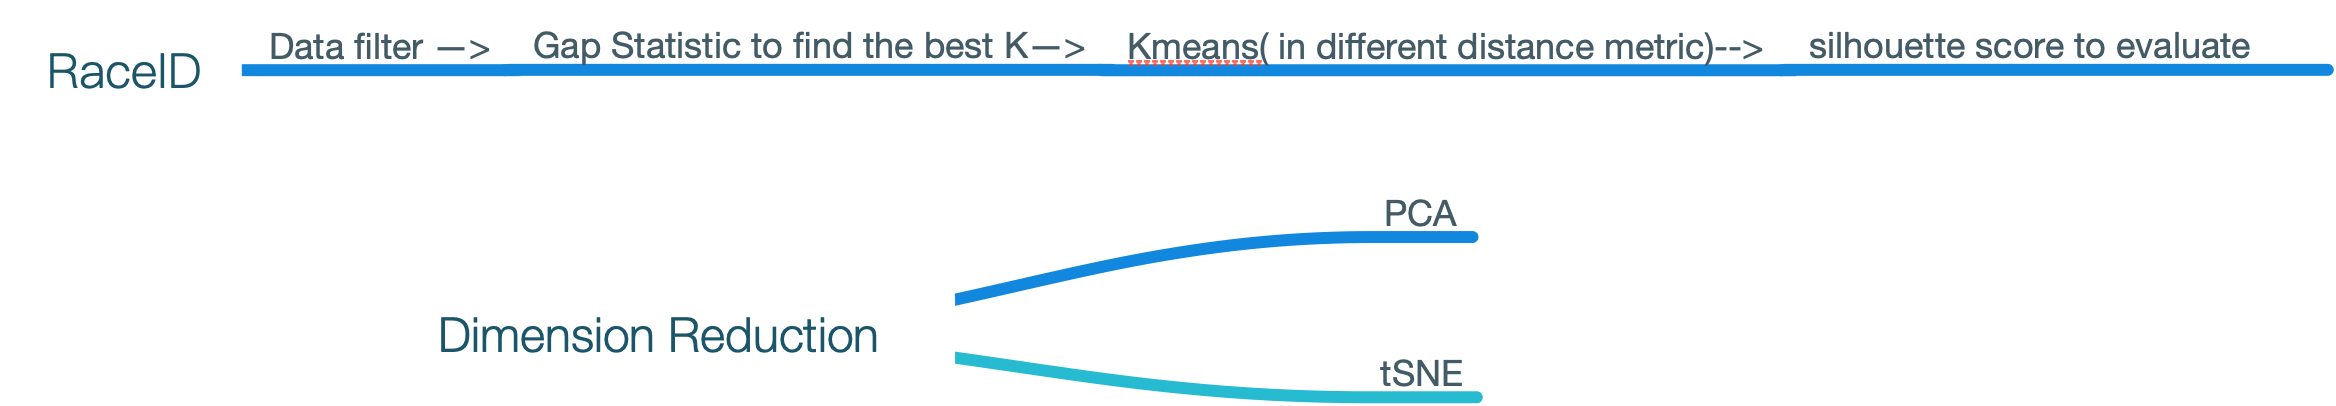
\includegraphics[width=0.4\textwidth]{fig2/workflow.png} 
\caption{Workflow of RaceID.} 
\label{Fig.1}
\end{figure}
\end{itemize}





\section{data}
The first dataset is found in original paper\(^1\) and the other is from Liying Yan\(^2\). Both of this data is based on unique molecular identifier(UMI) which is a method that uses molecular tags to detect and quantify unique mRNA transcripts and the big value presents that the RNA express more.\\
\hspace*{0.2 cm}Datasets are sparse and sparsity can be regarded as a good characteristic when matrix calculations are required. RaceID uses median to normalize and scale the data which has not been adopted in most scaling algorithms although it does not destroy the sparsity:\[RaceID \ Scaling=\frac{data_{ij}}{\sum_i data_{ij}}*median\]

To improve this, original way is replaced by Log. The reason is that logarithm does not change the relative relationships among data but compresses the scale of the variables. For distance-based clustering methods such as K-means, feature scaling impacts distance measure between cells. For example, if one of the features has a broad range of values, the Euclidean distance will be dominated by this particular feature. Thus, the ranges of all features should be normalized so that each feature contributes almost equally to the final distance. On the other hand, Log is the most powerful scaling tool as far as scRNA-seq data is considered. For example, SC3, BISCUIT and NMF all use Log.\\
\hspace*{0.2 cm}For data filtering, meaningless and insignificant RNA should be filtered by setting threshold: \\
Fiter RNA:
 \[\# (RNA>ThresholdOfExpression) > ThresholdOfNumbers \] 
 which will filter the housekeeping genes.\\
 Filter cell:\\
 \[(\sum RNA )< Threshold\]
 which express too less.

 \begin{figure}[H] 
\centering
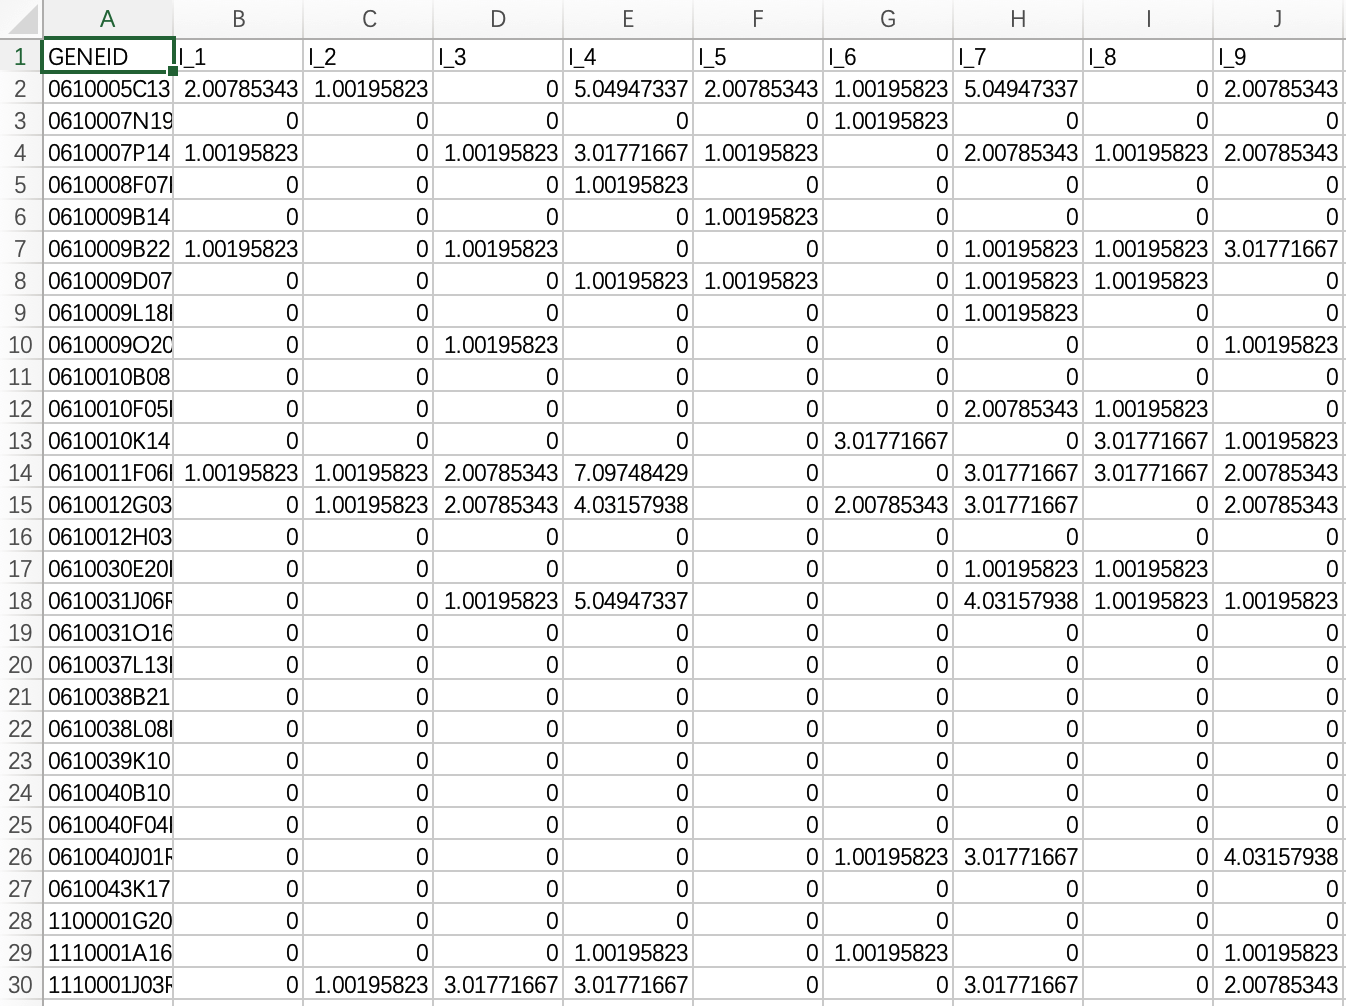
\includegraphics[width=0.4\textwidth]{fig2/data1.png} 
\caption{Data format of RaceID. Column presents cells and rows presents rows. Each number stands for UMI(unique molecular identifier) of each RNA in each cell.} 
\label{Fig.2}
\end{figure}






\section{Clustering}
The main purpose of RaceID is using clustering algorithms to find a special cluster which can present a rare cell type. K-means is used in RaceID with applying different metrics such as Euclidean, Spearman and Pearson. All of these metrics use different methods to calculate the distance between each points which means the similarity of points can be gotten from different ways. Certainly, the results will be varied among different metrics.\\
\hspace*{0.2 cm} K-means is known as as a  non-convex problem which  always converges to a local optimal solution without choosing a proper K and initial centers. To find the best K, gap statistic is used to evaluate the performance and estimate the best K.\[Gap_n(k)=E(logW^*)-logW\]
W presents the sum of distance of each point  after normalized while W\(^*\) is the distance of sampled data. The core idea of gap statistic is Monte Carlo which samples enough random points between the range of origin dataset for several times.  Gap value estimate the performance of clustering in each K abstractly by contrast the real data with sampled data in normal distribution. Higher gap value means in such K condition, the outcome of K-means using K clusters has a great difference with the clusters in null reference distribution and it presents a better performance. The estimate of the optimal clusters will be value that maximize the gap statistic.In Fig.3, the detailed process of  gap statistic is introduced.\\
\hspace*{0.2 cm} However, gap statistic's time complexity can be higher when user choose more samples and sampling for more times to get better and more accurate estimation. So, parallel calculation is adopted to accelerate and will be discussed in \(\uppercase\expandafter{\romannumeral5}\).\\
\hspace*{0.2 cm} Since gap statistic is a random algorithm, the outcome can change with different random seeds used in sampling.
 \begin{figure}[H] 
\centering
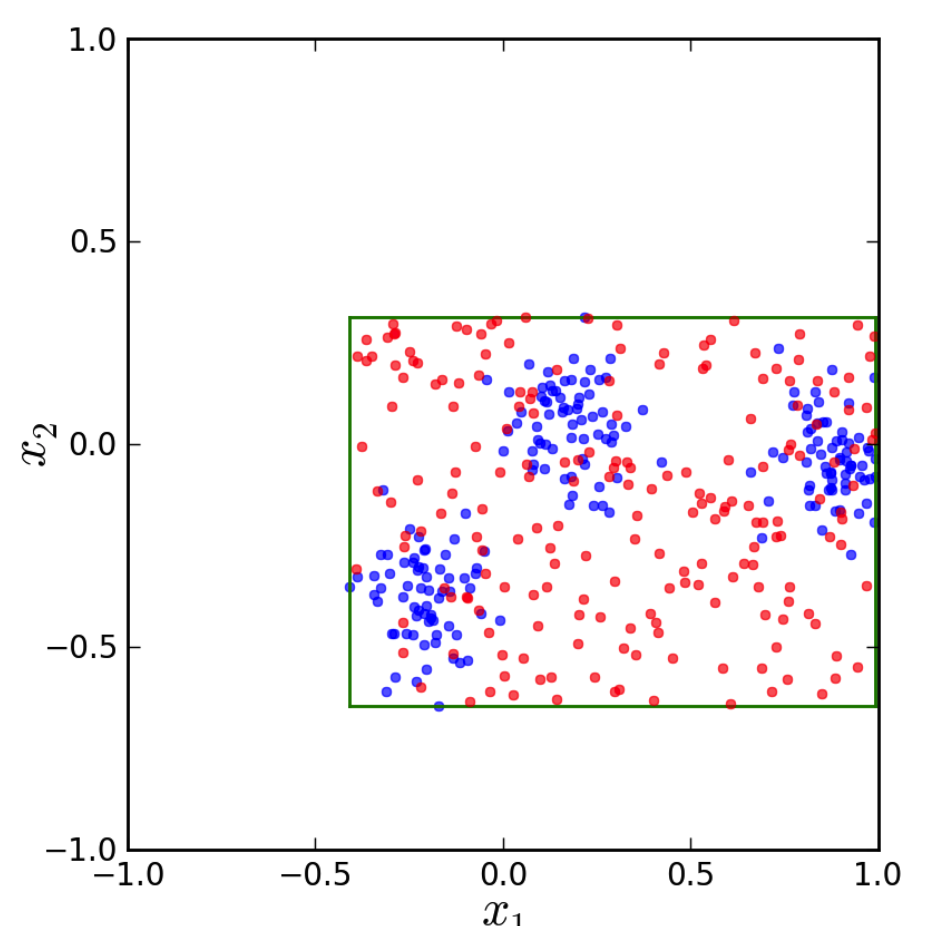
\includegraphics[width=0.4\textwidth]{fig2/gap1.png} 
\caption{Gap statistic in 2-dimension. Using blue points to present the real data set and red points stands for random sample data with Gaussian distribution.The gap statistic compares the total within intra-cluster variation for different values of k with their expected values under null reference distribution of the data. The estimate of the optimal clusters will be value that maximize the gap statistic. } 
\label{Fig.2}
\end{figure}

 \begin{figure}[H] 
\centering
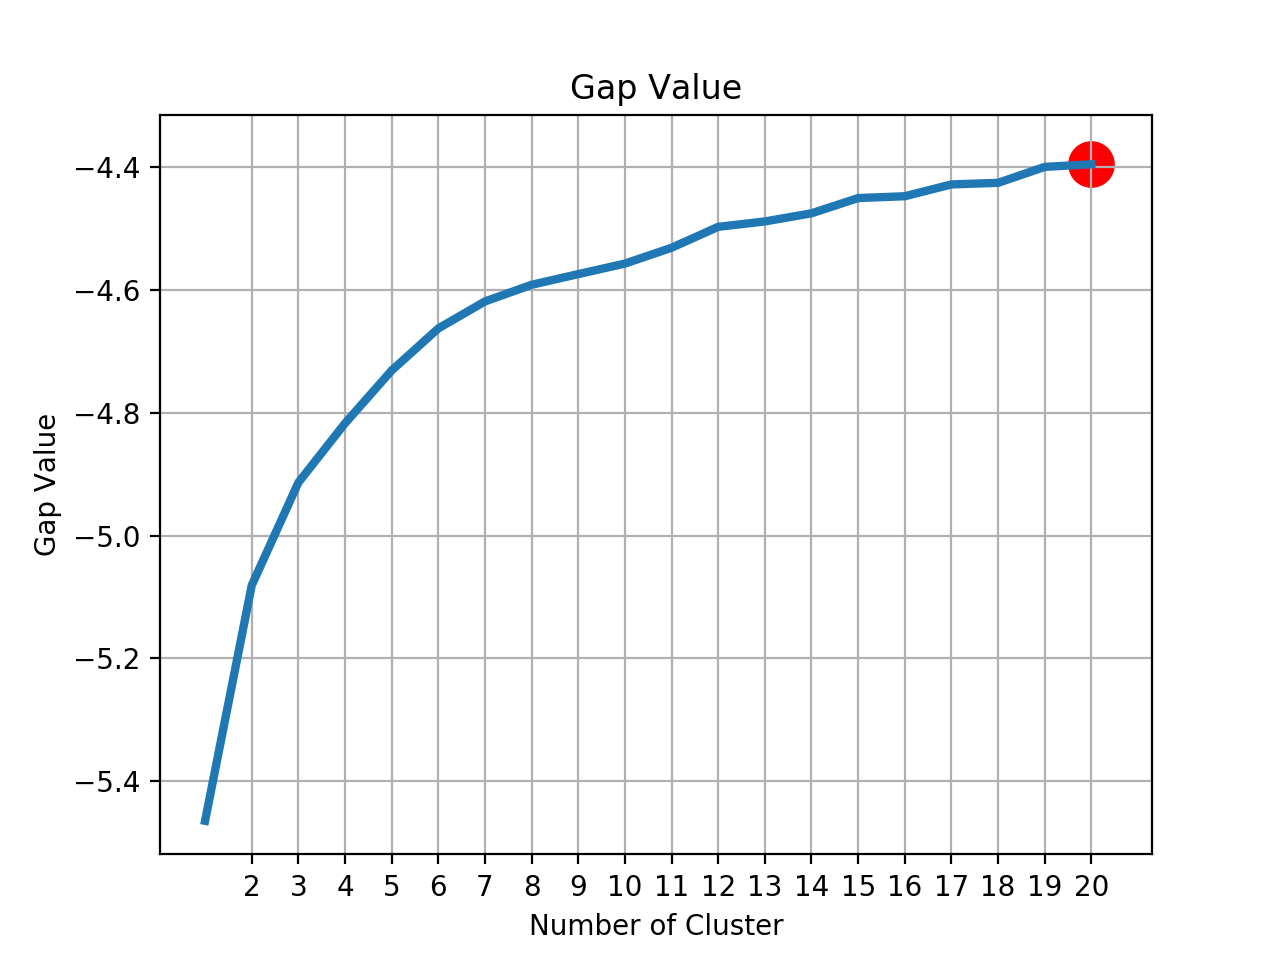
\includegraphics[width=0.4\textwidth]{fig2/gap2.png} 
\caption{It is the results of my experiments under \(max_K=20.\)} 
\label{Fig.4}
\end{figure}

 \begin{figure}[H] 
\centering
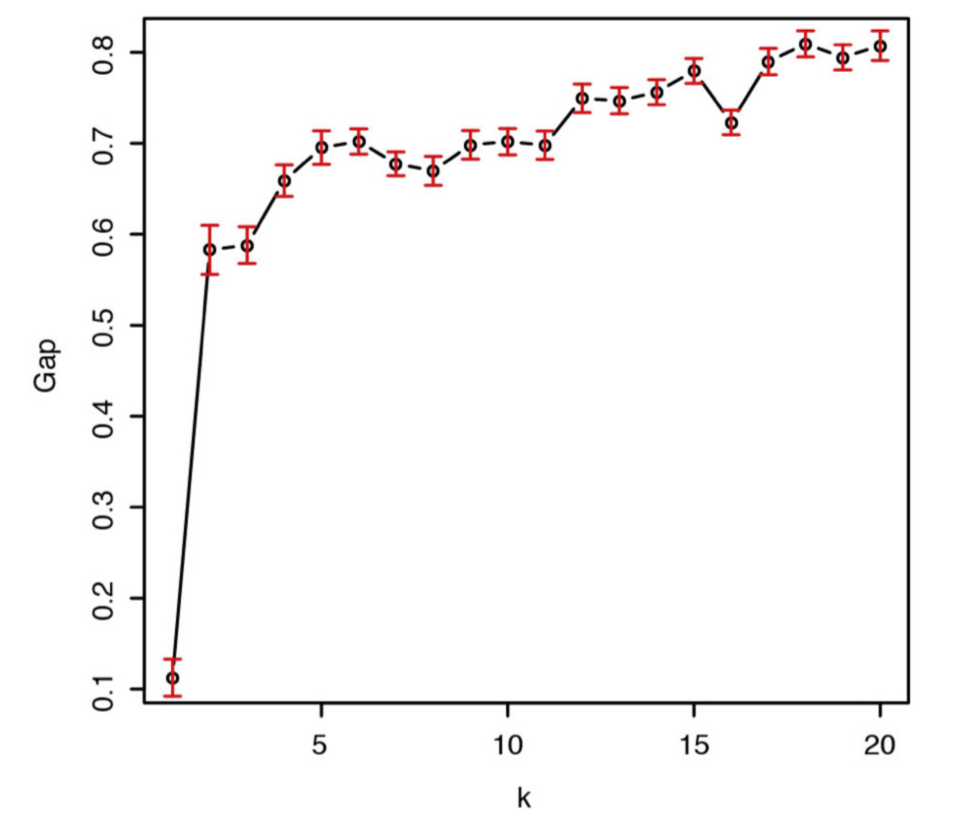
\includegraphics[width=0.4\textwidth]{fig2/gap3.png} 
\caption{ It is the original  results of RaceID under \(max_K=20\).} 
\label{Fig.5}
\end{figure}











\section{Dimension reduction and visualization}
The main dimension reduction algorithms can be classified into two types, the one for linear data, the other for nonlinear and even manifold. Principal components analysis(PCA) and t-distributed stochastic neighbor embedding(t-SNE) are adopted in RaceID.\\
\hspace*{0.2 cm} PCA is widely used in linear data ming which helps to get the linear characteristics and expose the inner information. The main idea of PCA is singular value decomposition(SVD) and choose the eigenvectors which corresponds to the maxima eigenvalues. Along these chosen eigenvectors, the data can project in the direction with biggest weight.\[X(data)=U\Sigma V^T\]
However, the results of PCA is terrible in RNA-seq data. The reason is that the data is not linear, even biologists can not explain the meaning of linear combinations of these dimensions in which presents the single RNA's expression.\\
\hspace*{0.2 cm} t-SNE is a manifold learning algorithm which uses a manifold model to keep the characteristic in locality by decreasing  the weight of points which is far.\\
\hspace*{0.2 cm}The similarity of data point \(x_j\) to datapoint \(x_i\) is the conditional probability  ,\(P_{j|i}\), that \(x_i\) would pick \(x_j\) at its neighbor if neighbors  were picked in proportion to their probability density under a Gaussian centered at \(x_i\). \(\sigma_i\) is the variance of the Gaussian distribution that is centered on datapoint \(x_i\).
\[P_{j|i}=\frac{\exp(-||x_i-x_j||^2 /2{\sigma_i}^2)}{\sum_k \exp(-||x_i-x_k||^2 /2{\sigma_i}^2)}\]
\hspace*{0.2 cm}Dimension reduction can be regarded as a process in which data in high dimension is mapped into the data in low dimension. \(Q_{j|i}\) is the similarity of \(y_i\) and \(y_j\) where \(y_i\) corresponds to \(x_i\) and \(y_j\) is from previous \(x_j\). We set the variance of Gaussian that is employed in the computation of the conditional probability \(Qj|i\) to \(\frac{1}{\sqrt{2}}\). Setting the variance in low dimension only changes the scale without any other side effect.
\[Q_{j|i}=\frac{\exp(-||y_i-y_j||^2)}{\sum_k \exp(-||y_i-y_k||^2 )}\]
\hspace*{0.2 cm}Finally, SNE minimize the sum of Kullback-Leibler divergence s over all data points which can estimate the mismatch between  two sets.
\[C=\sum_i KL(P_i||Q_i)=\sum_i\sum_jp_{j|i}log\frac {p_{j|i}}{q_{j|i}} \]
\hspace*{0.2 cm} \(\sigma_i\) is the last parameter to select. SNE defines a parameter named perplexity and  performs a binary search for the value of \(\sigma_i\) that produces a \(P_i\) with a fixed perplexity.
\[Perp(P_i)=2^{H(P_i)}\]
\(H(P_i)\) is Shannon entropy of \(P_i\) measured in bits:
\[H(P_i)=-\sum_j p_{j|i} \log_2{p_{j|i}} \]
After trying, choose a fixed perplexity.
 
 



\begin{figure}[H] 
\centering
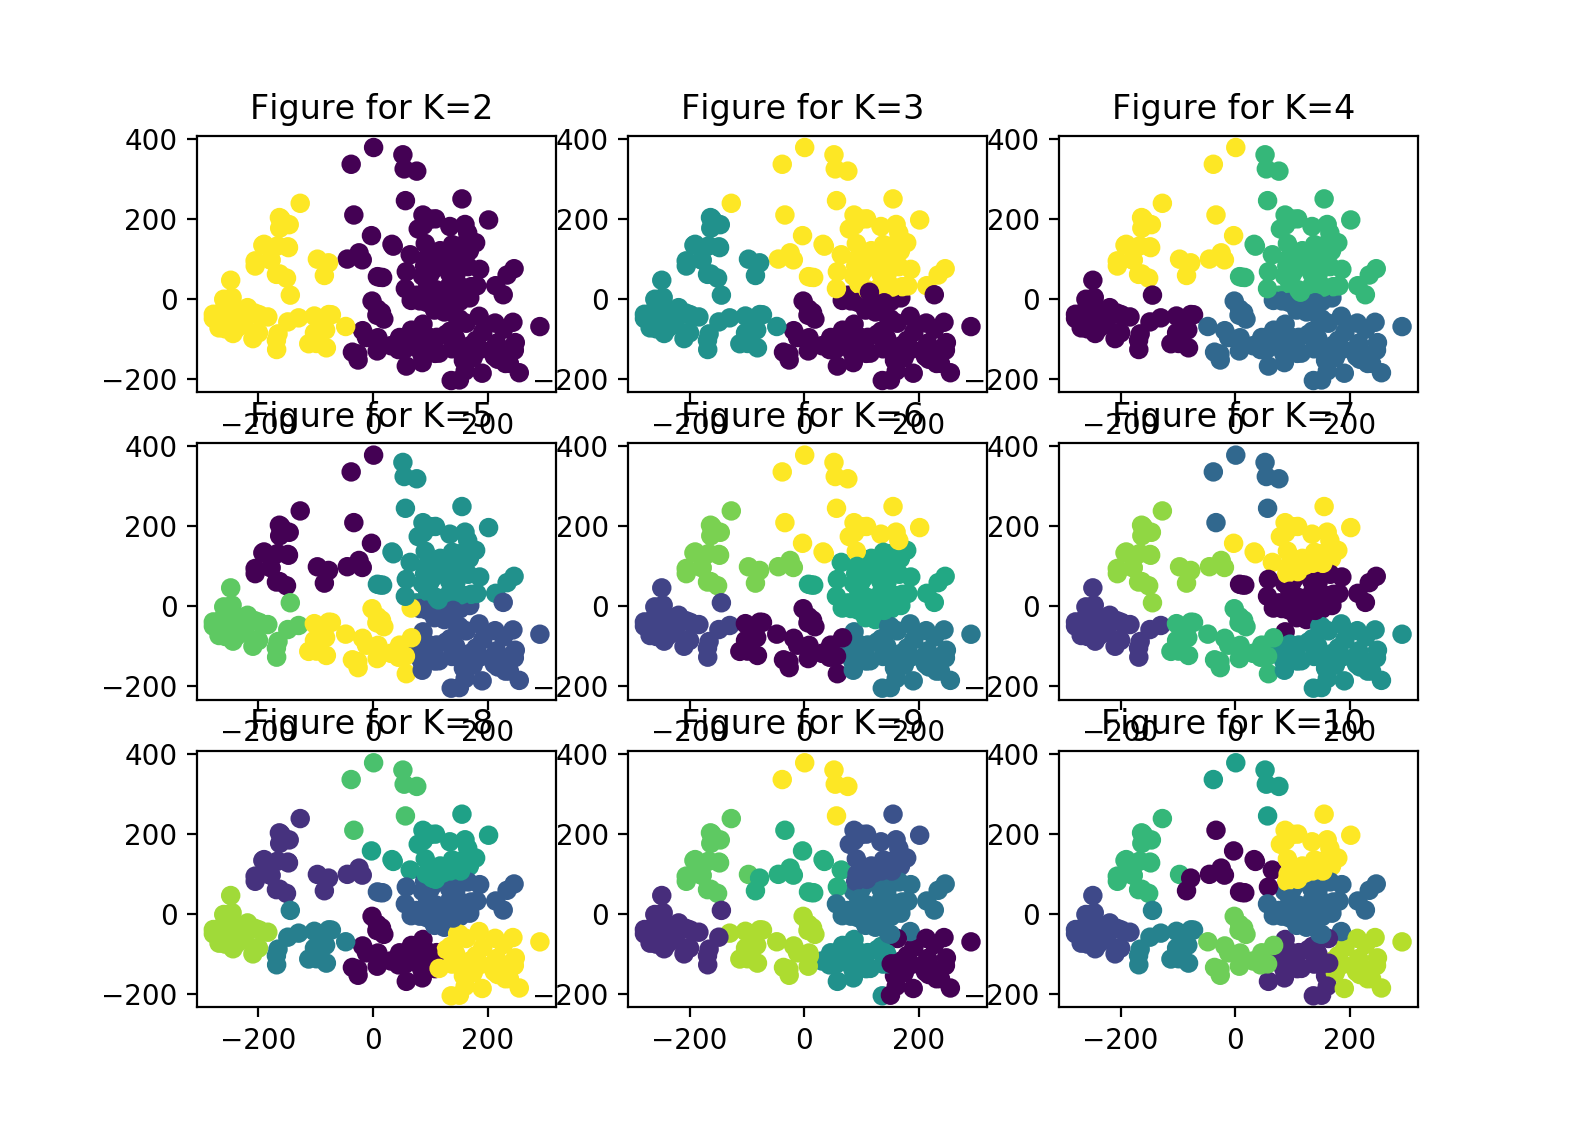
\includegraphics[width=0.4\textwidth]{fig2/pca.png} 
\caption{The results of 2-dimension clustering after PCA in \(max_K=10\). Different clusters are presented in different colors. Obviously, points gather together and hard to cluster. } 
\label{Fig.6}
\end{figure}


\begin{figure}[H] 
\centering
\includegraphics[width=0.4\textwidth]{fig2/tsne.png} 
\caption{ The t-SNE results from my expriment in 2-dimension with perplexity=29.8.  Different colors presents different clusters, the outcome looks better than PCA's. } 
\label{Fig.7}
\end{figure}

\begin{figure}[H] 
\centering
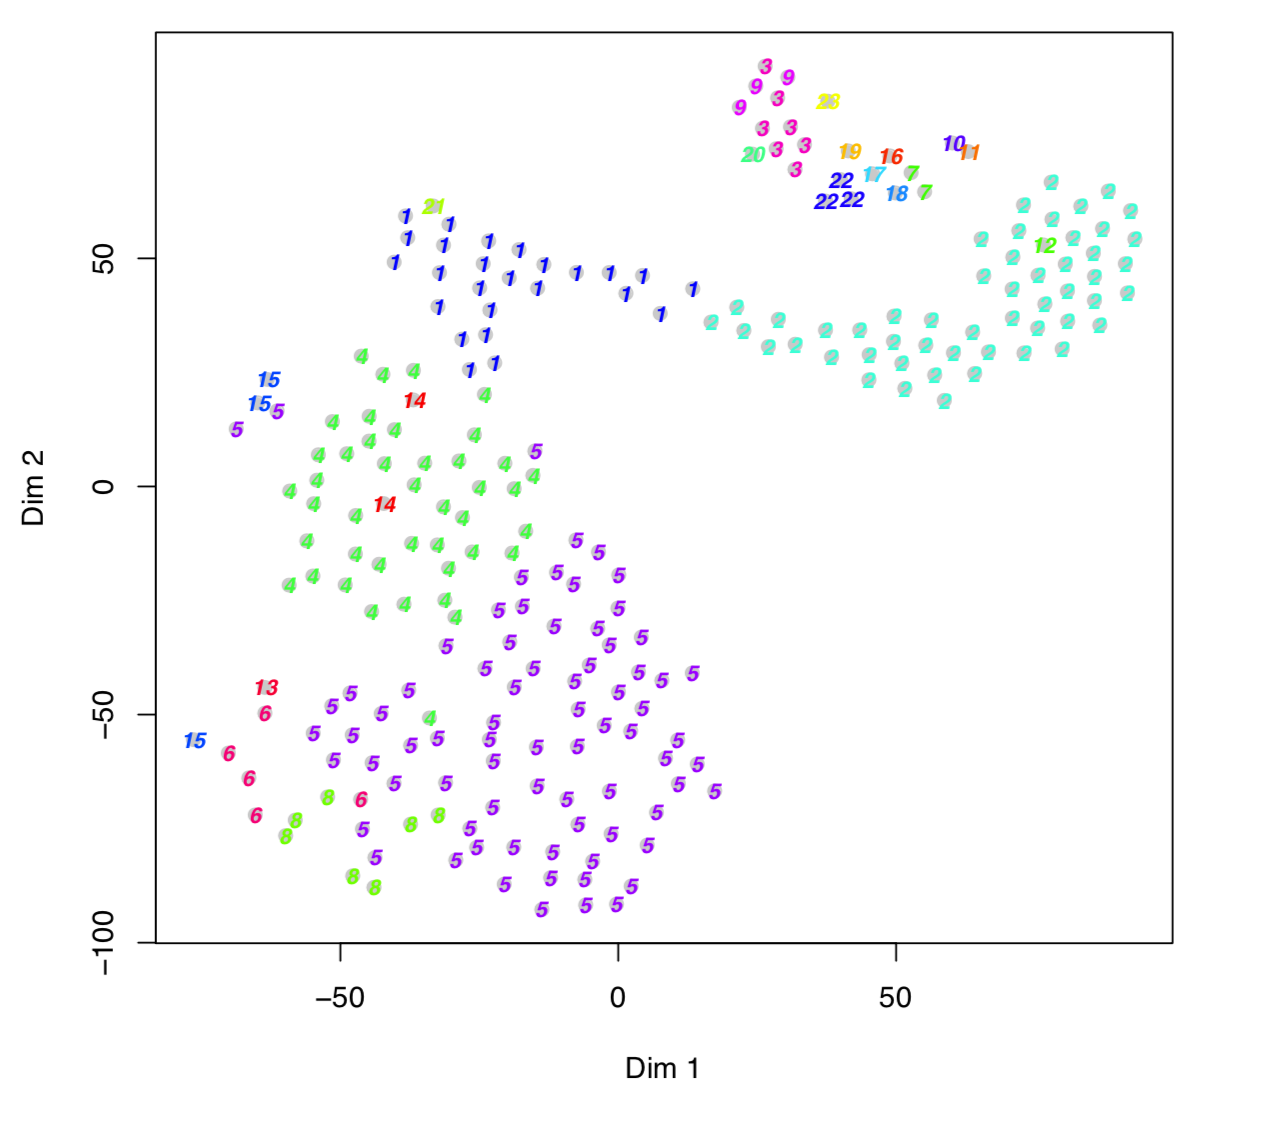
\includegraphics[width=0.4\textwidth]{fig2/tsne2.png} 
\caption{The t-SNE results from RaceID in 2-dimension with default perplexity=30.} 
\label{Fig.8}
\end{figure}





\section{Paralle programming}
To optimize and accelerate the calculation, parallel programming is comprehensively applied in multi-threads computers. MapReduce is the most famous parallel model published in 2008. I put MapReduce model in my algorithm which helps to accelerate getting gap value and best K. In loop, each iteration is despatched to a child-thread and all of these threads calculate in the same data simultaneously. After the calculation done, all the outputs are gathered to store in a same place.
\begin{figure}[H] 
\centering
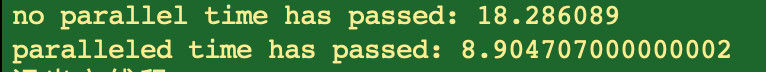
\includegraphics[width=0.4\textwidth]{fig2/parallel.png} 
\caption{ The performance of parallel calculation. The first line printed the time used without multi-threads and the second line presents the time used in parallel. The environments to calculate these two results are same. The same work finished in R needs 14.2576s that costs more 60\(\%\) time.} 
\label{Fig.9}
\end{figure}

	






\
\

\
\


\section{Reference}

\bibliographystyle{IEEEtran}
\bibliography{Reference}
[1]\emph{Single-cell messenger RNA sequencing reveals rare intestinal cell types}, Dominic Gru, Anna Lyubimova, Lennart Kester

[2]\emph{Single-cell RNA-Seq profiling of human preimplantation embryos and embryonic stem cells}, Liying Yan, Mingyu Yang, Hongshan Guo, Lu Yang

[3]\emph{Estimating the number of clusters in a data set via gap statistic}, Robert Tibshirani, Guenther Weather

[4]\emph{Visualizing data using t-SNE}, Laurens van der Maaten, Geoffery Hinton

[5]\emph{Principal component analysis},SvanteWold, Kim Esbensen, Paul Geladi

[6]\emph{k-means++: The advantages of careful seeding},D Arthur, S Vassilvitskii

[7]\emph{MapReduce: simplified data processing on large clusters}, J Dean, S Ghemawat 
\end{document}


